\documentclass{article}
\usepackage{amsmath}
\usepackage{amsfonts}
\usepackage{geometry}
\usepackage{listings}
\usepackage{enumitem}
\usepackage{graphicx}
\usepackage{comment}

\geometry{top=1in,bottom=1in,left=1in,right=1in}

\lstset{
	basicstyle=\ttfamily\small,
	breaklines=true,
	frame=single,
	xleftmargin=15pt,
	xrightmargin=15pt,
	columns=flexible,
}

\title{COMP3013 2024 Fall\\Assignment 2}
\author{Qiao Yichang}
\date{11.29}

\begin{document}
\maketitle

Q1. Convert the following ER diagram into logical schemas. (30pt)

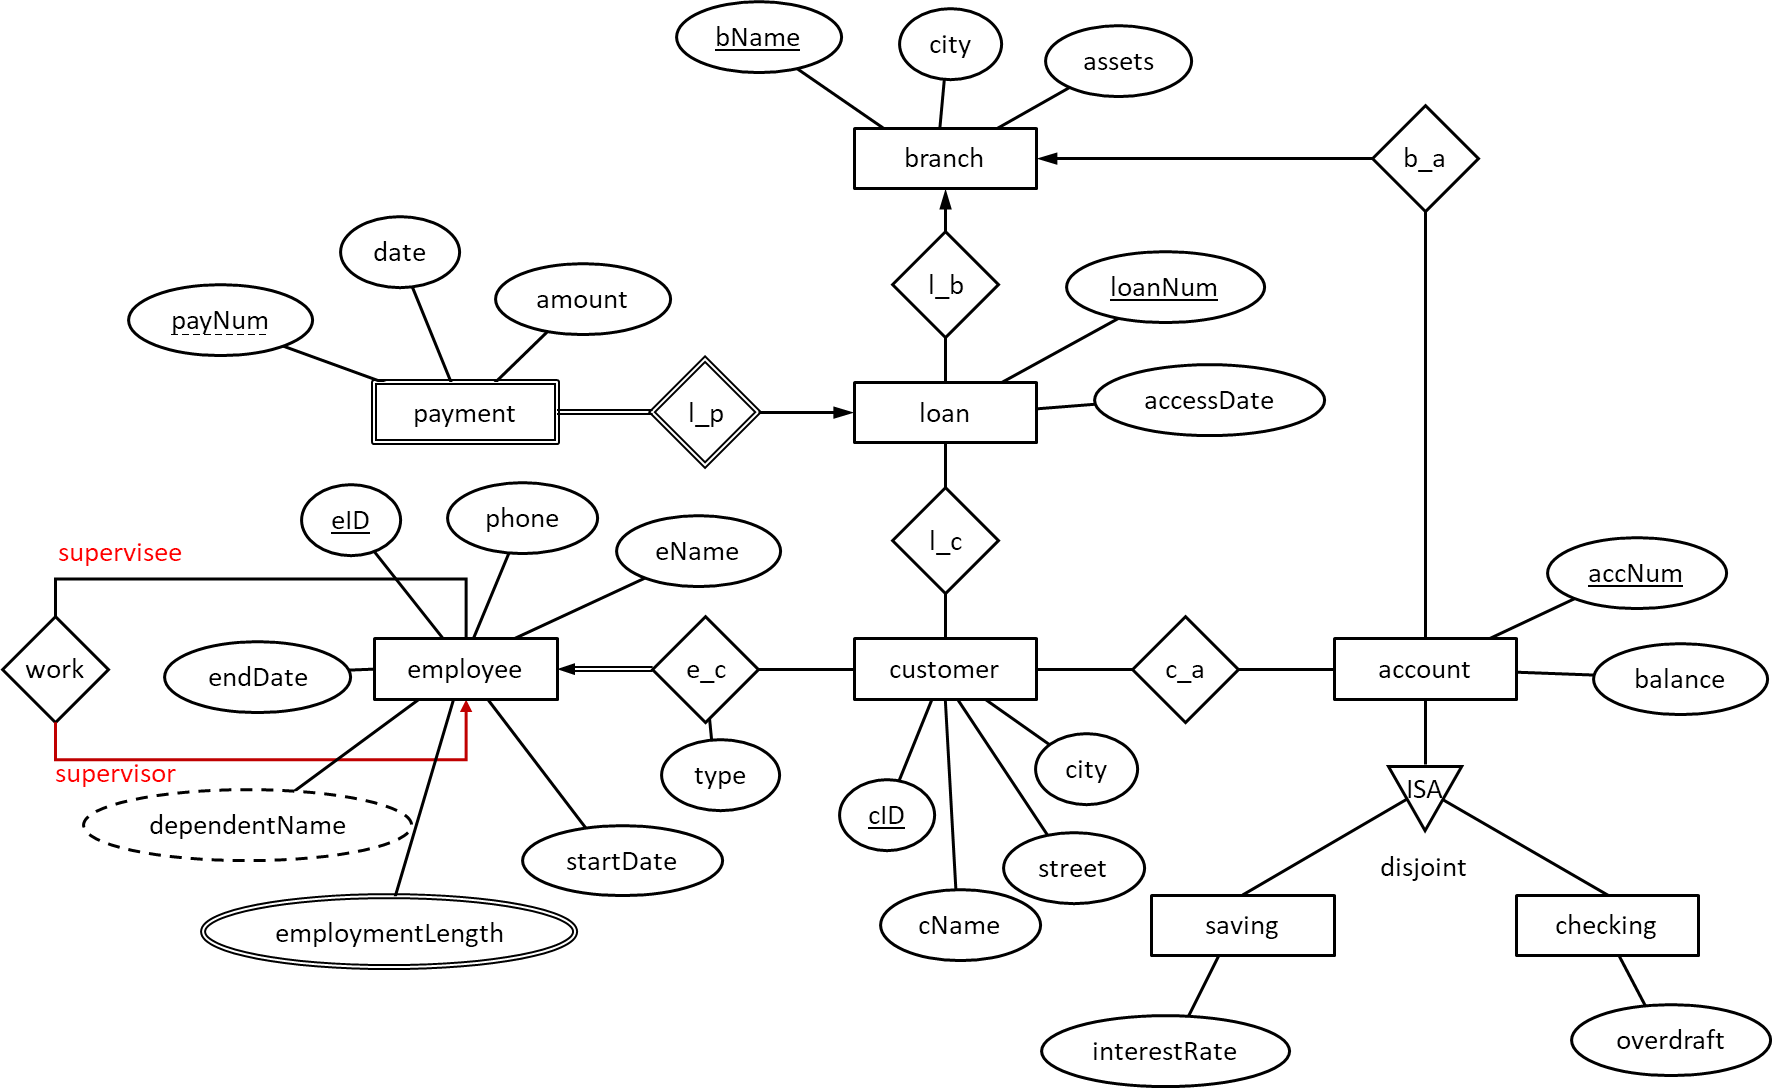
\includegraphics[width=5.90551in,height=3.62598in]{./image2.png}

The schema of a database for public transportation companies is as
follows. Keys are underlined.

\begin{itemize}
\item
  \(company = (\underline{cID},cname,address,phone)\)
\item
  \(route = (\underline{rID},departure,arrival,cID)\)


// \(cID\) is a foreign key to \(company.cID\).
\end{itemize}
\begin{itemize}
\item
  \(vehicle = (\underline{plateNum},model,capacity,manufacturer,cID)\)


// \(cID\) is a foreign key to \(company.cID\).
\end{itemize}
\begin{itemize}
\item
  \(driver = (\underline{dID},name,\ gender,age,cID)\)


// \(cID\) is a foreign key to \(company.cID\).
\end{itemize}
\begin{itemize}
\item
  \(serve = (\underline{rID,plateNum})\)


// \(rID\) is a foreign key to \(route.rID\).

// \(plateNum\) is a foreign key to \(vehicle.plateNum\).
\end{itemize}
\begin{itemize}
\item
  \(drive = (\underline{plateNum},dID)\)


// \(dID\) is a foreign key to \(diver.dID\).

// \(plateNum\) is a foreign key to \(vehicle.plateNum\).

\end{itemize}


\section*{Answer:}

\begin{itemize}
	\item \(branch = (\underline{biName}, city, assets, accNum, loanNum)\)
		\(\text{// } accNum \text{ is a foreign key to } account.accNum\).
		\(\text{// } loanNum \text{ is a foreign key to } loan.loanNum\).
	\item \(loan = (\underline{loanNum}, accessDate)\) \\
	
\end{itemize}

\begin{itemize}
	\item \(payment = (\underline{payNum}, date, amount)\) \\
\end{itemize}

\begin{itemize}
	\item \(employee = (\underline{eID}, eName, phone, startDate, endDate, biName, work)\) \\
	\(\text{// } biName \text{ is a foreign key to } branch.biName\). \\
	\(\text{// } eID \text{ is a foreign key to } employee.eID\).
\end{itemize}

\begin{itemize}
	\item \(customer = (\underline{cID}, cName, city, employmentLength, dependentName)\)
\end{itemize}

\begin{itemize}
	\item \(account = (\underline{accNum}, balance, type, biName)\) \\
	\(\text{// } biName \text{ is a foreign key to } branch.biName\).
\end{itemize}

\begin{itemize}
	\item \(saving = (\underline{accNum}, interestRate)\) \\
	\(\text{// } accNum \text{ is a foreign key to } account.accNum\).
\end{itemize}

\begin{itemize}
	\item \(checking = (\underline{accNum}, overdraft)\) \\
	\(\text{// } accNum \text{ is a foreign key to } account.accNum\).
\end{itemize}

\begin{itemize}
	\item \(L\_c = (\underline{loanNum, cID})\) \\
	\(\text{// } loanNum \text{ is a foreign key to } loan.loanNum\). \\
	\(\text{// } cID \text{ is a foreign key to } customer.cID\).
\end{itemize}

\begin{itemize}
	\item \(L\_p = (\underline{loanNum, payNum})\) \\
	\(\text{// } loanNum \text{ is a foreign key to } loan.loanNum\). \\
	\(\text{// } payNum \text{ is a foreign key to } payment.payNum\).
\end{itemize}

\begin{itemize}
	\item \(e\_c = (\underline{eID, cID}, type)\) \\
	\(\text{// } eID \text{ is a foreign key to } employee.eID\). \\
	\(\text{// } cID \text{ is a foreign key to } customer.cID\).
\end{itemize}


\begin{itemize}
	\item \(c\_a = (\underline{cID, accNum})\) \\
	\(\text{// } cID \text{ is a foreign key to } customer.cID\). \\
	\(\text{// } accNum \text{ is a foreign key to } account.accNum\).
\end{itemize}



Q2. Write a query for each following question. Assuming students' name
and instructors' name are unique. (10pt for each)

\begin{enumerate}
\def\labelenumi{\alph{enumi})}
\item
  Find the number of vehicles owned by ``Xinhe'' (company name).
  
  \begin{verbatim}
  	SELECT COUNT(*) AS num_vehicles
  	FROM Vehicles
  	WHERE company_name = 'Xinhe';
  \end{verbatim}
  
\item
  Find the companies who owns more than 10 vehicles. Show the company
  names and number of vehicles owned by each.
  
  \begin{verbatim}
  	SELECT company_name, COUNT(*) AS num_vehicles
  	FROM Vehicles
  	GROUP BY company_name
  	HAVING COUNT(*) > 10;
  \end{verbatim}
\item
  Find the route which is served by more vehicles than other routes.
  Show the departure and the arrival of the route.
  
  \begin{verbatim}
  	SELECT departure, arrival
  	FROM Routes
  	WHERE route_id = (
  	SELECT route_id
  	FROM Vehicles
  	GROUP BY route_id
  	ORDER BY COUNT(*) DESC
  	LIMIT 1
  	);
  \end{verbatim}
\item
  A driver retires at age 65 for males or at age 60 for females. Remove
  retired drivers from the database.
  
  \begin{verbatim}
  	DELETE FROM Drivers
  	WHERE (gender = 'Male' AND birth_date <= DATE_SUB(CURDATE(), INTERVAL 65 YEAR))
  	OR (gender = 'Female' AND birth_date <= DATE_SUB(CURDATE(), INTERVAL 60 YEAR));
  \end{verbatim}
\item
  The company ``ZhuhaiGongjiao'' (company name) opens a new route from
  ``UIC'' (departure) to ``Gongbei'' (destination). The company will
  assign any vehicle manufactured by ``BYD'' to the new route. Add
  correct records to the database.
  
  \begin{verbatim}

  	INSERT INTO Routes (departure, arrival)
  	VALUES ('UIC', 'Gongbei');
  	

  	SET @new_route_id = LAST_INSERT_ID();
  	

  	UPDATE Vehicles
  	SET route_id = @new_route_id
  	WHERE company_name = 'ZhuhaiGongjiao'
  	AND manufacturer = 'BYD';
  \end{verbatim}
\end{enumerate}


Q3. Implement the above logical design in SQL. You need to select
suitable data types and link foreign keys properly. (10 pt)

\section*{Answer:}
\subsection*{Table Definitions}

\begin{enumerate}
	\item \textbf{Vehicles Table}
	\begin{lstlisting}[language=SQL]
		CREATE TABLE Vehicles (
		vehicle_id INT PRIMARY KEY,         
		company_name VARCHAR(100) NOT NULL,   
		manufacturer VARCHAR(100),           
		model VARCHAR(100),                  
		route_id INT,                         
		FOREIGN KEY (route_id) REFERENCES Routes(route_id)
		);
	\end{lstlisting}
	
	\item \textbf{Routes Table}
	\begin{lstlisting}[language=SQL]
		CREATE TABLE Routes (
		route_id INT PRIMARY KEY AUTO_INCREMENT, 
		departure VARCHAR(100) NOT NULL,         
		arrival VARCHAR(100) NOT NULL            
		);
	\end{lstlisting}
	
	\item \textbf{Drivers Table}
	\begin{lstlisting}[language=SQL]
		CREATE TABLE Drivers (
		driver_id INT PRIMARY KEY,             
		first_name VARCHAR(100) NOT NULL,         
		last_name VARCHAR(100) NOT NULL,          
		gender CHAR(1) CHECK (gender IN ('M', 'F')), 
		birth_date DATE NOT NULL,               
		vehicle_id INT,                           
		FOREIGN KEY (vehicle_id) REFERENCES Vehicles(vehicle_id)
		);
	\end{lstlisting}
	
	\item \textbf{Companies Table}
	\begin{lstlisting}[language=SQL]
		CREATE TABLE Companies (
		company_name VARCHAR(100) PRIMARY KEY,    
		company_address VARCHAR(255),             
		contact_number VARCHAR(20)                 
		);
	\end{lstlisting}
	
	\item \textbf{Manufacturers Table}
	\begin{lstlisting}[language=SQL]
		CREATE TABLE Manufacturers (
		manufacturer_id INT PRIMARY KEY AUTO_INCREMENT,  
		manufacturer_name VARCHAR(100) NOT NULL,         
		country VARCHAR(100)                            
		);
	\end{lstlisting}
	
	\item \textbf{Route\_Vehicle Assignment Table (Many-to-Many Relationship)}
	\begin{lstlisting}[language=SQL]
		CREATE TABLE Route_Vehicle (
		route_id INT,               
		vehicle_id INT,             
		PRIMARY KEY (route_id, vehicle_id),
		FOREIGN KEY (route_id) REFERENCES Routes(route_id),
		FOREIGN KEY (vehicle_id) REFERENCES Vehicles(vehicle_id)
		);
	\end{lstlisting}
\end{enumerate}
\begin{comment}
	\subsection*{Explanation of Design}
	
	\begin{itemize}
		\item \textbf{Vehicles Table}: Contains information about the vehicles, with \texttt{vehicle\_id} as the primary key. The \texttt{company\_name} indicates the company that owns the vehicle, and \texttt{route\_id} links the vehicle to a specific route via a foreign key to the \texttt{Routes} table.
		\item \textbf{Routes Table}: Stores information about the routes, including a unique \texttt{route\_id}, departure, and arrival locations.
		\item \textbf{Drivers Table}: Contains driver details, with \texttt{driver\_id} as the primary key. Each driver is linked to a vehicle through \texttt{vehicle\_id} (foreign key). The \texttt{gender} field has a constraint to ensure that the value is either 'M' or 'F'.
		\item \textbf{Companies Table}: Stores company information such as \texttt{company\_name}, address, and contact details. \texttt{company\_name} is the primary key.
		\item \textbf{Manufacturers Table}: Stores manufacturer details for the vehicles. \texttt{manufacturer\_id} is the primary key, and it stores the name and country of the manufacturer.
		\item \textbf{Route\_Vehicle Table}: A junction table to handle the many-to-many relationship between routes and vehicles. A vehicle can be assigned to multiple routes, and a route can have multiple vehicles.
	\end{itemize}
	
	\subsection*{Foreign Key Relationships}
	
	\begin{itemize}
		\item \textbf{Vehicles Table} references \textbf{Routes} using \texttt{route\_id}.
		\item \textbf{Drivers Table} references \textbf{Vehicles} using \texttt{vehicle\_id}.
		\item \textbf{Route\_Vehicle Table} is used to link vehicles and routes with a many-to-many relationship.
		\item \textbf{Vehicles Table} also references \textbf{Companies} indirectly through the \texttt{company\_name}.
	\end{itemize}
\end{comment}
Q4. The above schema is converted from an ER diagram which has
\(company\), \(route\), \(vechile\), and \(driver\) as entity sets;
\(serve\) and \(drive\) as relationship sets. What are the constraints
on the two relationship sets? (10 pt)

\section*{Answer:}

\begin{itemize}
	\item \textbf{Entities}: 
	\begin{itemize}
		\item Company
		\item Route
		\item Vehicle
		\item Driver
	\end{itemize}
	\item \textbf{Relationships}: 
	\begin{itemize}
		\item Serve (between Company and Route)
		\item Drive (between Driver and Vehicle)
	\end{itemize}
\end{itemize}

Based on the schema and relationship sets, the constraints on the relationships are as follows:

\subsection*{1. Serve Relationship (between Company and Route)}
The \textbf{Serve} relationship connects the entities \textbf{Company} and \textbf{Route}, indicating that a company is responsible for operating a route.

\textbf{Constraints on the Serve Relationship}:
\begin{itemize}
	\item \textbf{Cardinality}: A company can serve multiple routes, and a route can be served by one or more companies. This is a \textbf{many-to-many} relationship.
	\item \textbf{Participation Constraints}:
	\begin{itemize}
		\item \textbf{Total Participation}: A route must be served by at least one company (if the route exists, it must have a company assigned to it).
		\item \textbf{Partial Participation}: A company may serve zero or more routes (it’s possible that a company may not serve any routes).
	\end{itemize}
	\item \textbf{Foreign Keys}: 
	\begin{itemize}
		\item \textbf{company\_name} (references the Company entity)
		\item \textbf{route\_id} (references the Route entity)
	\end{itemize}
\end{itemize}

\subsection*{2. Drive Relationship (between Driver and Vehicle)}
The \textbf{Drive} relationship connects the entities \textbf{Driver} and \textbf{Vehicle}, indicating that a driver is assigned to drive a specific vehicle.

\textbf{Constraints on the Drive Relationship}:
\begin{itemize}
	\item \textbf{Cardinality}: A vehicle can be driven by multiple drivers, and a driver can be assigned to multiple vehicles. This is a \textbf{many-to-many} relationship.
	\item \textbf{Participation Constraints}:
	\begin{itemize}
		\item \textbf{Total Participation}: Every driver must be assigned to at least one vehicle. A driver cannot exist without being assigned to a vehicle.
		\item \textbf{Partial Participation}: A vehicle may not necessarily have a driver assigned at any given time (this could be the case for new vehicles or during non-operational hours).
	\end{itemize}
	\item \textbf{Foreign Keys}: 
	\begin{itemize}
		\item \textbf{driver\_id} (references the Driver entity)
		\item \textbf{vehicle\_id} (references the Vehicle entity)
	\end{itemize}
\end{itemize}
\begin{comment}
	\subsection*{Summary of Constraints}
	\begin{itemize}
		\item \textbf{Serve Relationship}:
		\begin{itemize}
			\item \textbf{Cardinality}: Many-to-many (a company can serve multiple routes, and a route can be served by multiple companies).
			\item \textbf{Participation}: 
			\begin{itemize}
				\item \textbf{Route}: Total participation (every route must be served by at least one company).
				\item \textbf{Company}: Partial participation (a company may not serve any routes).
			\end{itemize}
			\item \textbf{Foreign Keys}: 
			\begin{itemize}
				\item \textbf{company\_name} (references the Company)
				\item \textbf{route\_id} (references the Route)
			\end{itemize}
		\end{itemize}
		\item \textbf{Drive Relationship}:
		\begin{itemize}
			\item \textbf{Cardinality}: Many-to-many (a vehicle can be driven by multiple drivers, and a driver can drive multiple vehicles).
			\item \textbf{Participation}: 
			\begin{itemize}
				\item \textbf{Driver}: Total participation (every driver must be assigned to at least one vehicle).
				\item \textbf{Vehicle}: Partial participation (a vehicle may not have a driver assigned).
			\end{itemize}
			\item \textbf{Foreign Keys}: 
			\begin{itemize}
				\item \textbf{driver\_id} (references the Driver)
				\item \textbf{vehicle\_id} (references the Vehicle)
			\end{itemize}
		\end{itemize}
	\end{itemize}
\end{comment}

\end{document}
